\documentclass[a4paper,11pt]{article}
\usepackage[hidelinks]{hyperref}
\usepackage{graphicx}
\usepackage[utf8]{inputenc}
\usepackage[T1]{fontenc}
\usepackage[portuguese]{babel}
\usepackage{indentfirst}
\usepackage{mathtools}
\date{\today}
\author{{\bf Engenharia Informática}\\Sérgio Batista - 31500\\João Calhau - 31621\\André Figueira - 31626\\Luís Zurrapa - 32330}
\title{{\bf Universidade de Évora}\\Intrudução à Probabilidade e Estatistica\\Relatório do Trabalho Prático}

\begin{document}
 
\maketitle

\begin{figure}[ht!]
\centering

\includegraphics[width=90mm]{estatistica}
\label{overflow}
\end{figure}

\newpage
\tableofcontents

\newpage
\section{Introdução}

\newpage
\section{Questões}
\subsection{Questão 1:}
\indent Ano: Variável quantitativa discreta\\
\indent Região: Variável qualitativa nominal\\
\indent AcessoNet: Variável quantitativa discreta

\subsubsection{Variável Ano}

%\begin{figure}[ht!]
%\centering
%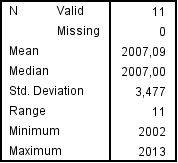
\includegraphics[width=45mm]{tabela1(Ano)}
%\caption{Tabela SPSS para as 3 regiões}
%\label{overflow}
%\end{figure}


\newpage
\subsubsection{Variável Região}
%insert image here
\subsubsection{Variável AcessoNet}

%\begin{figure}[ht!]
%\centering
%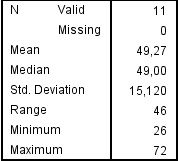
\includegraphics[width=35mm]{tabela1(AcessoNet)}
%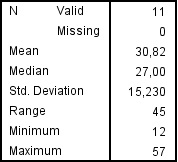
\includegraphics[width=35mm]{tabela2(AcessoNet)}
%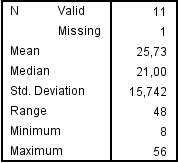
\includegraphics[width=35mm]{tabela3(AcessoNet)}
%\caption{Tabela SPSS para as regiões EUarea, PT e GR, respectivamente}
%\label{overflow}
%\end{figure}

\newpage
\subsection{Questão 2:}

\newpage
\subsection{Questão 3:}
\subsubsection{a)}
\indent A média e o desvio-padrão antes calculados assumem os mesmos valores que as estimativas pontuais da média e do desvio-padrão.
\newline

\subsubsection{b)}
\begin{figure}[ht!]
\centering
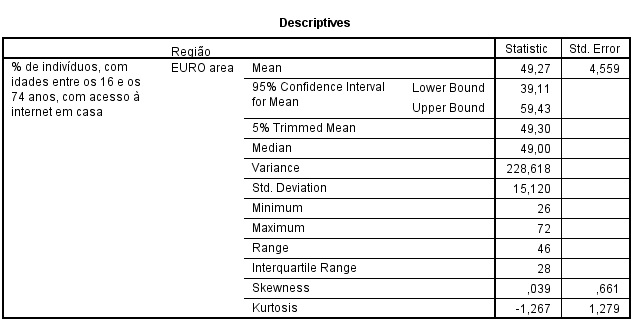
\includegraphics[width=76mm]{IC(EUarea)}
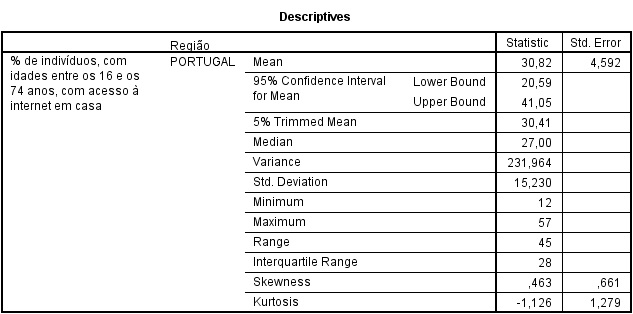
\includegraphics[width=76mm]{IC(PT)}
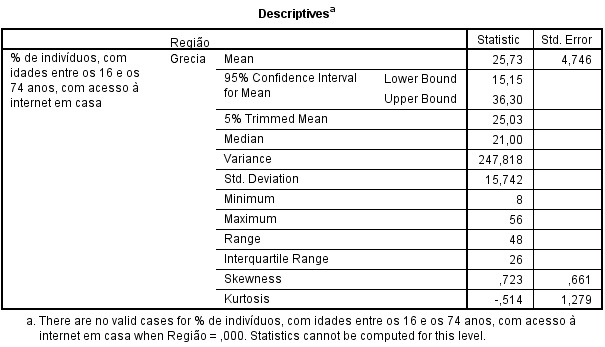
\includegraphics[width=76mm]{IC(GR)}
\label{overflow}
\end{figure}

\noindent Para um intervalo de confiança de 95\% para a média tiramos, destas tabélas, que:\\
Para a Euro area, temos um limite superior de 59,43 e um limite inferior de 39,11\\
Para Portugal, temos um limite superior de 41,05 e um limite inferior de 20,59.\\
Para a Grécia, temos um limite superior de 36,30 e um limite inferior de 15,15.\\

\newpage
\subsubsection{c)}

\begin{figure}[ht!]
\centering
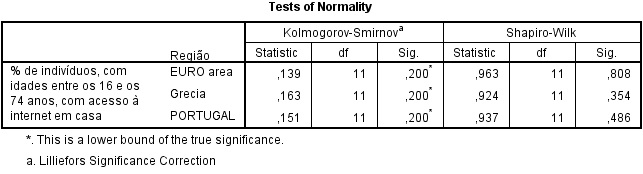
\includegraphics[width=100mm]{p-value}
\label{overflow}
\end{figure}
\noindent $H_{0}$: "As asmostras provêm de uma população gaussiana"  \ vs $H_{1}$: "As amostras não provêm de uma população gaussiana"\\

\noindent Rejeitamos $H_{0}$ se $\alpha \geq$ p-value\\

\noindent Por esta tabela podemos concluir que, a um nivel de significancia de 5\%, ($\alpha$=0,05), visto que para as 3 regiões o $\alpha$ é sempre menor que o p-value, não rejeitamos o $H_{0}$, logo podemos dizer que as amostras provêm de populações gaussianas.
\newline

\subsubsection{d)}
Euro Area vs Portugal:
\begin{figure}[ht!]
\centering
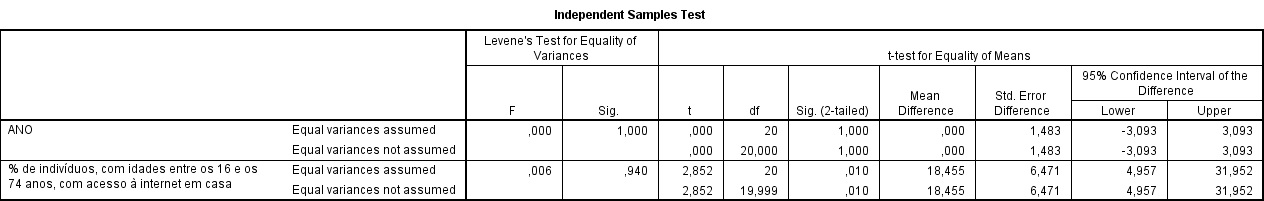
\includegraphics[width=130mm]{EUareaVsPT}
\label{overflow}
\end{figure}



Euro Area vs Grécia:
\begin{figure}[ht!]
\centering
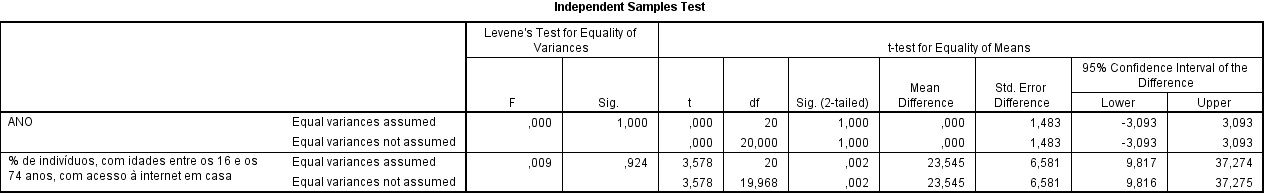
\includegraphics[width=130mm]{EUareaVsGR}
\label{overflow}
\end{figure}


\newpage
Portugal vs Grécia:
\begin{figure}[ht!]
\centering
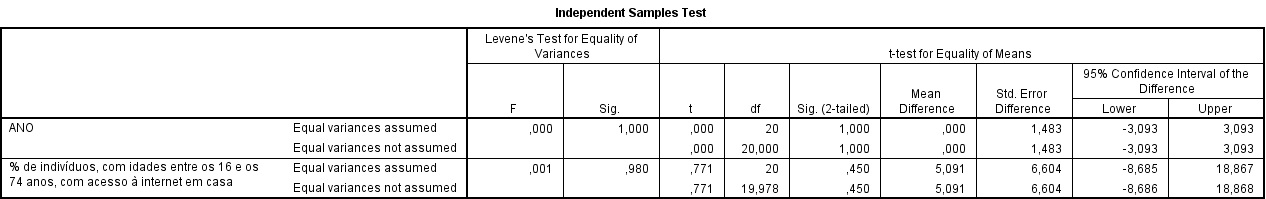
\includegraphics[width=130mm]{PTvsGR}
\label{overflow}
\end{figure}


\newpage
\section{Materiais e métodos}
\subsection{Materiais:}


\subsection{Métodos:}
\indent Para a resolução deste trabalho utilizamos vários métodos, desde o cálculo de medidas de tendência central e não central a assimetrias e achatamentos, incluindo entre estes medidas de dispersão e coeficientes de variação. Foram utilizados testes de hipótese e intervalos de confiança. Foi também necessário comparar médias e fazer regressões lineares, bem como interpertar p-values e testes de normalidade.\\
\indent Por fim determinaram-se os coeficientes de correlação e construíram-se as rectas de regressão dos minimos quadrados.

\newpage
\section{Análise dos resultados}
%insert stuff here

\newpage
\section{Conclusão}
\indent Com a realização deste trabalho pretendiamos como aspeto inicial começar a trabalhar com o software SPSS. Para utilizar de maneira mais eficaz este recurso utilizamos os conhecimentos aprendidos ao longo do ano.\\
\indent Tendo em conta isto podemos dizer que os objetivos que nos foram propostos para este trabalho foram cumpridos e que neste momento temos pelo menos as noções básicas deste software preparando-nos para qualquer neccessidade no futuro.\\
\indent Assim podemos concluir que ao longo deste trabalho...................

\end{document}